\documentclass[a4paper]{article}
\usepackage[dutch]{babel}
\usepackage{amsmath}
\usepackage{amssymb}
\usepackage{graphicx}
\usepackage{mathtools}
\usepackage{float}

\graphicspath{ {afbeeldingen/} }

\title{Numerieke Modellering en Benadering: Practicum 1}
\author{Ellen Anthonissen \and Marte Biesmans}
\date{vrijdag 21 april 2016}

\newcommand{\opgave}[1]{\section*{Opgave #1}}
\newcommand{\dx}{\Delta x}
\newcommand{\dy}{\Delta y}
\newcommand{\dz}{\Delta z}
\newcommand{\dt}{\Delta t}

\begin{document}
\maketitle

\opgave{1} %Marte
De Householder transformatiematrix
$$F=I - 2\frac{vv^*}{v^*v}$$
heeft als eigenwaarden $-1$ en $1$ en als eigenvectoren respectievelijk $v$ en $w$ met $w \perp v$. Deze resultaten zijn als volgt bekomen:
De Householder transformatiematrix $F$ is symmetrisch 
$$F^* = (I - 2\frac{vv^*}{v^*v})^* = I - 2\frac{vv^*}{v^*v} = F$$
en unitair
$$F^*F = FF^* = (I - 2\frac{vv^*}{v^*v})(I - 2\frac{vv^*}{v^*v}) = I - 4\frac{vv^*}{v^*v} + 4\frac{v(v^*v)v^*}{(v^{*}v)^2} = I.$$
Omdat $F$ unitair is, moeten de eigenwaarden van $F$ op de complexe eenheidscirkel gelegen zijn.
Omdat $F$ re\"eel en symmetrisch is, zijn de eigenwaarden re\"ele getallen.
Hieruit volgt dat de eigenwaarden enkel $\pm 1$ kunnen zijn.

Als we nu $Fv$ uitrekenen, bekomen we
$$Fv = v - 2\frac{vv^*}{v^*v}v = -v.$$
Hieruit volgt dat $v$ en eigenvector is bijhorende bij de eigenwaarde $-1$.
Neem nu $w$ met $w \perp v$ en we rekenen $Fw$ uit, dan bekomen we
$$Fw = w - 2\frac{vv^*}{v^*v}w = w,$$
want $v^*w = 0$. Hieruit volgt das $w$ een eigenvector is bijhorende bij de eigenwaarde $1$.

Geometrisch gezien komt dit overeen met een spiegeling over de $w$-as. Neem een vector $a$ en ontbind die in een compontent volgens de $v$-as en een component volgens de $w$-as. De component volgens de $v$-as zal vermenigvuldigt worden met $-1$ en die volgens de $w$-as met $1$. Zo bekomen we een spiegeling rond de $w$-as.

\opgave{2} %Marte
De functie Householder\_explicit wordt weergegeven in onderstaande MATLAB-code. Deze methode genereert de matrix $Q$ door na de impliciete methode een nieuwe loop uit te voeren. Deze loop is gebaseerd op de functie om het product $Qx$ te berekenen, met voor $x$ telkens een eenheidsvector.
$\backslash$
Na het expliciet berekenen van de QR-factorisatie van A, wordt de oplossing van het stelsel $Ax=b$ bekomen door $y = Q^*b$ en $x= R\backslash y$ te berekenen.

\lstinputlisting[
  style      = Matlab-editor,
  basicstyle = \mlttfamily,
]{Householder_explicit.m}

De functies Householder\_implicit en Apply\_Q zijn Hier onder weergegeven in MATLAB-code.
Na het berekenen van L en R en L toe te passen op b (noem deze vector y), wordt de oplossing van het stelsel $Ax=b$ bekomen door $x= R\backslash y$ te berekenen. 

\lstinputlisting[
  style      = Matlab-editor,
  basicstyle = \mlttfamily,
]{Householder_implicit.m}

\lstinputlisting[
  style      = Matlab-editor,
  basicstyle = \mlttfamily,
]{Apply_Q.m}

De tijd om het stelsel $Ax=b$ op te lossen met de expliciete en de impliciete methode worden respectievelijk weergegeven in tabel \ref{snelheid_exp} en tabel \ref{snelheid_imp}. Hier zien we dat de tijd om het stelsel op te lossen een orde-grootte kleiner is met de impliciete methode dan met de expliciete methode.

De ordegroottes van de relatieve fout $\lVert \delta x \rVert/\lVert x \rVert$ van de oplossing voor de expliciete en de impliciete methode worden respectievelijk weergegeven in tabel \ref{dx_exp} en tabel \ref{dx_imp}.
De ordegroottes van de verhouding van de norm van het residu op de norm van de b-vector $\lVert r \rVert/\lVert b \rVert$ van de oplossing voor de expliciete en de impliciete methode worden respectievelijk weergegeven in tabel \ref{rb_exp} en \ref{rb_imp}. Deze waarden vullen we nu in in de vergelijking
$$ \frac{\lVert \delta x \rVert}{\lVert x \rVert} \leq \kappa(A) \frac{\lVert r \rVert}{\lVert b \rVert}.$$
We zien hier dat het linkerlid van de ongelijkheid veel kleiner is dan het rechterlid naarmate $\kappa$ groter wordt. Voor $\kappa = 1$ zien we namelijk dat het linkerlid ongeveer gelijk is aan het rechterlid. Voor $\kappa = 10^8$ is er veel meer verschil tussen de twee leden. We zien zelfs dat wanneer $\kappa = 1$, de ongelijkheid niet meer helemaal klopt. Dit komt omdat de machine-precisie dan de beperkende factor wordt. We zien ook voor beide methodes dezelfde getallen, dus de mate van achterwaartse stabiliteit van de twee methodes is ongeveer dezelfde.

\begin{table}[H]
\begin{center}
\begin{tabular}{r|llc}
n $\backslash$ $\kappa$ & $1$ & $10^4$ & $10^8$ \\\hline
10 & 0,0044 & 0,0022 & 0,0025 \\
100 & 0,1883 & 0,1403 & 0,1306 \\
1000 & 28,2691 & 27,725 & 27,9583
\end{tabular}
\end{center}
\caption{De snelheid van de expliciete methode}
\label{snelheid_exp}
\end{table}

\begin{table}[H]
\begin{center}
\begin{tabular}{r|llc}
n $\backslash$ $\kappa$ & $1$ & $10^4$ & $10^8$ \\\hline
10 & 0,0050 & 0,0015 & 0,0013 \\
100 & 0,0115 & 0,0131 & 0,0163 \\
1000 & 7,9605 & 7,7967 & 7,8586
\end{tabular}
\end{center}
\caption{De snelheid van de impliciete methode}
\label{snelheid_imp}
\end{table}

\begin{table}[H]
\begin{center}
\begin{tabular}{r|llc}
n $\backslash$ $\kappa$ & $1$ & $10^4$ & $10^8$ \\\hline
10 & $10^{-16}$ & $10^{-13}$ & $10^{-9}$ \\
100 & $10^{-15}$ & $10^{-13}$ & $10^{-9}$ \\
1000 & $10^{-14}$ & $10^{-13}$ & $10^{-9}$
\end{tabular}
\end{center}
\caption{De ordegrootte van $\lVert \delta x \rVert/\lVert x \rVert$ van de expliciete methode}
\label{dx_exp}
\end{table}

\begin{table}[H]
\begin{center}
\begin{tabular}{r|llc}
n $\backslash$ $\kappa$ & $1$ & $10^4$ & $10^8$ \\\hline
10 & $10^{-16}$ & $10^{-13}$ & $10^{-9}$ \\
100 & $10^{-15}$ & $10^{-13}$ & $10^{-9}$ \\
1000 & $10^{-15}$ & $10^{-13}$ & $10^{-9}$
\end{tabular}
\end{center}
\caption{De ordegrootte van $\lVert \delta x \rVert/\lVert x \rVert$ van de impliciete methode}
\label{dx_imp}
\end{table}

\begin{table}[H]
\begin{center}
\begin{tabular}{r|llc}
n $\backslash$ $\kappa$ & $1$ & $10^4$ & $10^8$ \\\hline
10 & $10^{-16}$ & $10^{-13}$ & $10^{-9}$ \\
100 & $10^{-15}$ & $10^{-13}$ & $10^{-9}$ \\
1000 & $10^{-14}$ & $10^{-13}$ & $10^{-10}$
\end{tabular}
\end{center}
\caption{De ordegrootte van $\lVert r \rVert/\lVert b \rVert$ van de expliciete methode}
\label{rb_exp}
\end{table}

\begin{table}[H]
\begin{center}
\begin{tabular}{r|llc}
n $\backslash$ $\kappa$ & $1$ & $10^4$ & $10^8$ \\\hline
10 & $10^{-16}$ & $10^{-13}$ & $10^{-9}$ \\
100 & $10^{-15}$ & $10^{-13}$ & $10^{-10}$ \\
1000 & $10^{-14}$ & $10^{-13}$ & $10^{-10}$
\end{tabular}
\end{center}
\caption{De ordegrootte van $\lVert r \rVert/\lVert b \rVert$ van de impliciete methode}
\label{rb_imp}
\end{table}

\opgave{3} %Ellen

\opgave{4} %Marte
Neem een vector $x \in \mathbb{R}^n$. Schrijf $x$ als lineaire combinatie van de eigenvectoren van $A$ $q_1, q_2 \dots q_n$ met bijhorende eigenwaarden $\lambda_1, \lambda_2 \dots \lambda_n$:
$$ x = \sum_{j=1}^{n}a_jq_j,$$
dan is het Rayleigh quoti\"ent van $x$:
$$r(x) = \frac{\sum_{j=1}^{n}a_j^2q_j\lambda_j}{\sum_{j=1}^{n}a_j^2}.$$
Het Rayleigh quoti\"ent is onafhankelijk van de schaal van $x$, dus stel $\lVert a \rVert = \lVert \begin{bsmallmatrix} a_1&a_2&\dots&a_n\end{bsmallmatrix}^T \rVert = 1$, dan is $\sum_{j=1}^{n}a_j^2 = 1$. Dan wordt het Rayleigh quoti\"ent gelijk aan
$$r(x) = \sum_{j=1}^{n}a_j^2q_j\lambda_j.$$
Stel nu dat $\lambda_1 \geq \lambda_2 \geq \dots \geq \lambda_n$, dan is het Rayleigh quoti\"ent maxiaal voor $a = e_1$ met de waarde $\lambda_{max}$ en minimaal voor $a = e_n$ met de waarde $\lambda_{min}$. Dus het Rayleigh quoti\"ent bevint zich in het interval $\begin{bsmallmatrix}\lambda_{min},\lambda_{max}\end{bsmallmatrix}$.

Ook is het Rayleigh quoti\"ent een continu voor $a \neq 0$, dus elke waarde tussen $\lambda_{min}$ en $\lambda_{max}$ wordt bereikt voor een bepaalde vector $a$, dus ook voor een bepaalde vector $x$.

\opgave{5} %Ellen

\opgave{6} %Marte
We maken gebruik van de ongelijkheid
$$ \frac{\lVert e_n \rVert_A}{\lVert e_0 \rVert_A} \leq 2 \bigg(\frac{\sqrt{\kappa}-1}{\sqrt{\kappa}+1}\bigg)^n.$$
Voor $n=10$ wordt dit
$$ \frac{\lVert e_{10} \rVert_A}{\lVert e_0 \rVert_A} \leq 2 \bigg(\frac{\sqrt{\kappa}-1}{\sqrt{\kappa}+1}\bigg)^{10}. $$
Gebruik makende van de gegevens $\lVert e_0 \rVert_A = 1$ en $\lVert e_{10} \rVert_A = 2 \times 2^{-10}$, bekomen we
$$9 \leq \kappa.$$
We vinden dus een ondergrens voor $\kappa$.

Voor $n=20$ wordt de ongelijkheid
$$ \frac{\lVert e_{20} \rVert_A}{\lVert e_0 \rVert_A} \leq 2 \bigg(\frac{\sqrt{\kappa}-1}{\sqrt{\kappa}+1}\bigg)^{20}. $$
Gebruik makende van het gegeven $\lVert e_0 \rVert_A = 1$ en het berekende $9 \leq \kappa$, bekomen we
$$ \lVert e_{20} \rVert_A \leq 2 \times 2^{-20}.$$
We vinden dus een bovengrens voor $ \lVert e_{20} \rVert_A$.

\opgave{7} %Ellen

\opgave{8} %Ellen

\opgave{9} %Marte
De interlace eigenschap van een tridiagonale, symmetrische en re\"ele matrix $A$ luidt als volgt. Voor $A \in \mathbb{R}^{n \times n}$, en $A^{(1)}, A^{(2)}  \dots A^{(n)}$ de principale vierkante submatrices van dimensie $1, 2 \dots n$, geldt dat de eigenwaarden van deze submatrices interlacen. Dit wil zeggen dat $\lambda_j^{(k+1)} \leq \lambda_j^{(k)} \leq \lambda_{j+1}^{(k+1)}$. Als $A$ irreduceerbaar is (en dus geen nul heeft op een nevendiagonaal), dan worden de ongelijkheden stricte ongelijkheden.

Als voorbeeld nemen we de tridiagonale, symmetrische en re\"ele matrix
$$A = \begin{bmatrix} 
1 &5 &0 &0\\
5 &2 &6 &0 \\
0 &6 &3 &7\\
0 &0 &7 &4
\end{bmatrix}.$$
We zien duidelijk op figuur \ref{fig:oef9_1} dat de eigenwaarden van een principale submatrix tussen de eigenwaarden van de principale submatrix van een dimensie groter liggen.

\begin{figure}[H]
    \centering
    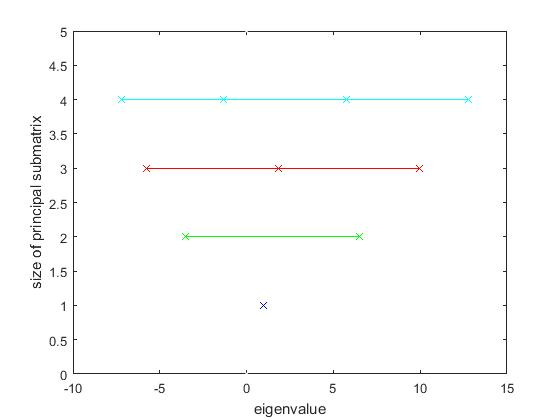
\includegraphics[width=0.7\textwidth]{oef9_1.jpg}
    \caption{De eigenwaarden van de opeenvolgende principale submatrices van A}
    \label{fig:oef9_1}
\end{figure}

\opgave{10} %Marte
Een algoritme in pseudo-code dat alle eigenwaarden van een symmetrische, tridiagonale en re\"ele matrix in het interval [a,b) berekent tot op een bepaalde tolerantie met behulp van de bisectie-methode, is te vinden in algoritme \ref{bisectie}.

\begin{algorithm}[H]
\centering
\caption{Bisectie-methode}
    \label{bisectie}
\begin{algorithmic}
\State{queue = [[a,b)]}
\While{queue niet leeg}
\State{Haal eerste interval uit de queue}
\State{$Sturm_{links}$ = \#tekenwisselingen in de Sturm-rij van A-linkergrens*I}
\State{$Sturm_{rechts}$ = \#tekenwisselingen in de Sturm-rij van A-rechtergrens*I}
\State{\#eigenwaarden = $Sturm_{rechts}$ - $Sturm_{links}$}
\State{midden = 0.5*(rechtergrens - linkergrens)}

\If {\#eigenwaarden == 1}
	\If{midden $<$ tolerantie}
		\State{Voeg linkergrens+midden toe als eigenwaarde}
	\Else
    \State {Voeg [linkergrens,linkergrens+midden] en [linkergrens+midden,rechtergrens] vooraan bij in de queue}
    \EndIf
\ElsIf {\#eigenwaarden $>$ 1}
        \State {Voeg [linkergrens,linkergrens+midden] en [linkergrens+midden,rechtergrens] vooraan bij in de queue}
\EndIf
\EndWhile
\end{algorithmic}
\end{algorithm}


Deze methode werd uitgeschreven in MATLAB (zie onderstaande code) en werd toegepast op enkele symmetrische, tridiagonale en re\"ele matrices.

\lstinputlisting[
  style      = Matlab-editor,
  basicstyle = \mlttfamily,
]{bisection.m}

Als eerste voorbeeld nemen we de tridiagonale, symmetrische en re\"ele matrix $A \in \mathbb{R}^{n \times n}$ met $n=4$.
$$A = \begin{bmatrix} 
1 &5 &0 &0 \\
5 &2 &6 &0 \\
0 &6 &3 &7 \\
0 &0 &7 &4 \\
\end{bmatrix}$$
Als we de eigenwaarden van deze matrix willen berekenen in het interval [-2,6) tot op een tolerantie $10^{-2}$, dan vinden we we eigenwaarden [-1,3359375; 5,7734375]. Deze komen overeen met de 'exacte' eigenwaarden [-1,32970777874292; 5,77851991186833] berekend met de functie eig($A$) van MATLAB. Als we beide resultaten afronden tot op twee cijfers na de komma, zien we inderdaad dat de eigenwaarden gevonden zijn tot op de gegeven absolute fout.

Een interessant testprobleem is een random symmetrische, tridiagonale en re\"ele matrix $B \in \mathbb{R}^{n \times n}$ MATLAB met $n = 100$. De diagonalen zijn berekend met de functie rand($n$) en rand($n-1$). We zoeken naar de eigenwaarden in het interval [0,1) tot op een tolerantie $10^{-2}$. De matrix waarmee dit getest is, wordt hier niet weergegeven omdat deze veel te groot is. Het interessante aan deze matrix is dat de eigenwaarden die tussen 0 en 1 gelegen zijn, meestal dichter bij elkaar liggen dan de opgegeven tolerantie. Het algoritme dat hierboven beschreven wordt, kan toch nog steeds onderscheid maken tussen de verschillende eigenwaarden. Zo vindt het bijvoorbeeld als eerste twee eigenwaarden 0,03515625 en 0,04296875 voor de eigenwaarden (berekend met de eig() functie van MATLAB) 0,0340437309188287 en 0,0441523470170203.

Een volgend interessant testprobleem wordt bekomen door eigenwaarden als grens te nemen. Theoretisch gezien mag de eigenwaarde die de rechtergrens voorstelt niet gevonden worden. Dit is echter soms toch het geval (zeker voor grote matrices). Dit komt doordat de elementen van de Sturm-rij opgesteld worden aan de hand van vorige elementen. Zo kunnen reken- en afrondingsfouten zich voortplanten.

Ook is er tijdens het testen opgevallen dat de gevraagde nauwkeurigheid niet altijd bereikt wordt voor alle eigenwaarden. Dit komt doordat wanneer de grens van een te onderzoeken interval dicht bij een eigenwaarde komt, de Sturm-rij van $A-xI$ slecht geconditioneerd is. Het laatste element ligt dan rond 0, waardoor er snel een tekenwissel te veel of te weinig is.


\end{document}
